\section{Floquetifying the colour code}\label{sec:floquetifying_colour_code}

We can apply the same ideas as in the last section to stabilizer codes
more interesting than the $\qcode{4, 2, 2}$ code.
In this section, we take this more interesting stabilizer code to be the colour code.
Or, more accurately, we take it to be the \textit{bulk} of the colour code -
i.e.\ ignoring the code's global topology (whether it lives on a torus, or is planar).
A discussion of global topology is deferred to
\Cref{subsec:floquetifying_colour_code_beyond_bulk} at the end of this section,
and continued in detail in \Cref{sec:floquetifying_colour_code_beyond_bulk}.

\subsection{The bulk}\label{subsec:floquetifying_colour_code_bulk}

The $\mathit{6.6.6}$ \textit{colour code} is a stabilizer code defined on a honeycomb lattice, with qubits placed at vertices.
We write $v \in f$ to mean that a vertex $v$ is incident to a hexagonal face $f$.
For any such face $f$, we define weight-six Paulis $X_f = \prod_{v \in f} X_v$ and $Z_f = \prod_{v \in f} Z_v$.
On a torus, the code is defined by the measurement schedule
$\MMM = [\langle \{Z_f: \text{face $f$}\} \rangle,~ \langle \{X_f: \text{face $f$}\} \rangle]$.
On a planar geometry, slightly different Paulis are measured at the boundaries~\cite{ColourCodeBoundariesAndTwists}.

\begin{figure}[t]
    \centering
    
\includegraphics[width=\linewidth]{figures/floquetifying/colour_code/zx_rewritten}
    \caption{
        Two equivalent ZX-diagrams for a patch of the colour code at three consecutive timesteps.
        Ideally we'd draw vertical wires connecting each column of patches,
        like we were able to do for the $\qcode{4, 2, 2}$ code in the last section,
        but doing this renders the diagrams pretty much unreadable.
        Instead, we draw very small vertical wires going up and/or down from certain spiders, labelled by letters.
        These letters define how a wire going vertically upwards in one layer is actually connected to
        a wire coming vertically downwards from the layer above it;
        wires labelled by the same letter are connected.
    }
    \label{fig:colour_code_rewritten}
\end{figure}

As before, we start with a ZX-diagram of the colour code over multiple timesteps;
see the left hand side of \Cref{fig:colour_code_rewritten}.
We then unfuse every spider into four or five spiders to get the diagram on the right of the figure.
In these diagrams, grey hexagons, bars and integers, as well as letter labels and coloured wires, all have no meaning in the ZX-calculus; they're just visual aids.
In the diagram on the right, wires within grey bars correspond to weight-two measurements,
while all other wires correspond to qubit world-lines.
The focus is on a single qubit's world-line, which we've coloured purple;
we can see that it's only involved in measurements with four other qubits,
which we've coloured orange, pink, blue and brown.
It turns out that all qubit world-lines have this property of only interacting with four other qubits.
Furthermore, these interactions are such that the qubits of the new code can be laid out on a square lattice.
So henceforth we'll label qubits of the new code with a pair of integer coordinates $(x, y)$.

The grey bars labelled by integers denote the timesteps of the new code.
These are well-defined;
picking any qubit world-line and following it up the page
while noting down the integer label of every grey bar it crosses produces an increasing sequence.
For example, doing this for the purple qubit produces the contiguous sequence $[0, 1, 2, \ldots]$.
As before, we can view all one-legged spiders as halves of single-qubit measurements.
The pattern repeats after every two timesteps of the old code (the colour code);
one can see this by noting that the bottom and top of the diagram are identical,
up to a translation in space and an increase by 13 in the labels of the grey bars.
In other words, this new code has a period of 13.

\begin{figure}[t]
    \centering
    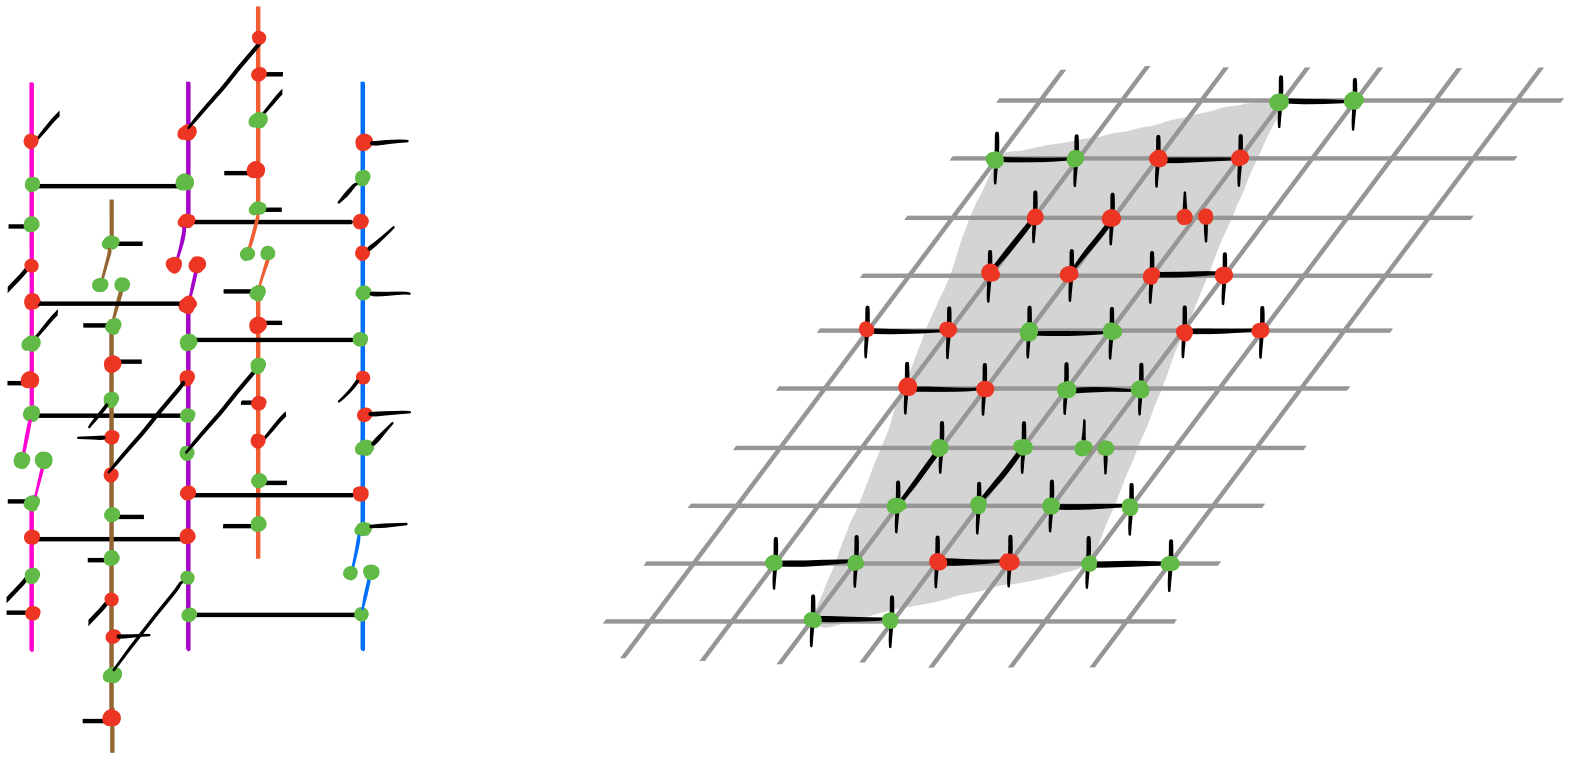
\includegraphics[width=\linewidth]{figures/floquetifying/colour_code/floquetified/measurement_schedule}
    \caption{
        Left: measurements undergone by a single qubit and its four nearest neighbours over one full period of 13 timesteps.
        Right: One `tile' of one timestep of the measurement schedule in the bulk of the Floquetified colour code.
        Here the grey lines are \textit{not} ZX-diagram wires -
        they are just visual aids that show this all sits on a square lattice.}
    \label{fig:floquetified_colour_code_measurement_schedule}
\end{figure}
Again, we can now write down the measurements that each qubit undergoes at each timestep.
In \Cref{fig:floquetified_colour_code_measurement_schedule},
we show a ZX-diagram of this, focused on the purple qubit from \Cref{fig:colour_code_rewritten}.
Each qubit undergoes essentially the same pattern of measurements in each period.
Specifically, whatever measurement qubit $(x, y)$ undergoes at timestep $t$,
qubit $(x, y+1)$ undergoes it at time $t-2$, but with the roles of $Z$ and $X$ exchanged.
Likewise for the remaining neighbours $(x+1, y)$, $(x, y-1)$ and $(x-1, y)$,
but at times $t-8$, $t+2$ and $t+8$ respectively.
Knowing this, we can then write down the measurement schedule for the bulk of the new code
(i.e.\ what measurements are happening at any single timestep).
This has a periodic structure; we draw a ZX-diagram for a single timestep $t$ and single `tile' of this on the right of \Cref{fig:floquetified_colour_code_measurement_schedule}.
To see the measurements happening across the whole bulk at this timestep, one should tile these grey rectangles across the square lattice.
That is, whatever measurement qubit $(x, y)$ undergoes at time $t$, qubits $(x+3, y+1)$ and $(x-2, y+8)$ undergo this too.
Then to get the measurements happening at the next timestep, one should translate the measurements from time $t$ by $(-1, -3)$.
That is, whatever measurement qubit $(x, y)$ undergoes at time $t$, qubit $(x-1, y-3)$ undergoes it at time $t+1$.
\begin{figure}[t]
    \centering
    
\includegraphics[width=\linewidth]{figures/floquetifying/colour_code/floquetified/detector}
    \caption{
        A detecting region in the colour code and the corresponding detecting region in the Floquetification.
        Again, grey lines are \textit{not} ZX-diagram wires -
        they are just a visual guide showing the square lattice.}
    \label{fig:detector_floquetified_colour_code}
\end{figure}

Detectors and logical operators can again not only be worked with algebraically,
but also graphically, via Pauli webs.
In \Cref{fig:detector_floquetified_colour_code} we show a detecting region in the colour code bulk and its image in the bulk of the new Floquet code.
The corresponding detector in the new code consists of 14 weight-two measurements and 4 single-qubit measurements, spread over 8 timesteps.
Every detector in the bulk of the new code is identical to this one,
up to a space-time translation and exchanging $Z$ and $X$.
Just as in the colour code, these detecting regions are tiled such that unique errors
violate unique sets of detectors, so decoding can be performed,
though we leave investigating specific decoding strategies to future work.
A similar exercise can be repeated for the logical operators;
one can draw the operating regions corresponding to the known logical operators of the colour code,
and see how these map to operating regions in the Floquetified code,
from which one can write down the new code's logical operators.

\subsection{Beyond the bulk}\label{subsec:floquetifying_colour_code_beyond_bulk}

The Floquetification process described above can be applied directly to planar colour codes,
and will lead to a new code that is itself planar.
But since the boundaries of the original code look different to the bulk,
extra work needs to be done to Floquetify these correctly.
Furthermore, the resulting Floquet code can exhibit a `drifting' behaviour,
which we discuss in more detail in \Cref{subsec:drift}.
There are potential perks of this behaviour - e.g.\ for removing leakage -
but it's also handy to have a code that doesn't drift.
One might think we could get around these two issues by starting with the colour code defined on a torus,
which has no boundaries to worry about.
But viewing our procedure as tilting the time direction in a ZX-diagram for a code,
as described in the last section,
we find we can only give well-defined new timesteps when the code we start with is planar -
this is discussed in more depth in \Cref{subsec:periodic_boundaries}.
Instead, if we want to avoid boundaries,
what we can do is Floquetify only the bulk,
which will give the bulk of a potential new Floquet code,
then see if placing this new bulk on a torus still encodes logical qubits.
In \Cref{subsec:colour_code} we apply the two ideas described above -
we Floquetify a planar colour code,
and place the Floquetified colour code bulk from this section on a torus.
